\chapter{Технологический раздел}
На сегодняшний день существует большое количество языков и технологий, используемых как для разработки серверной части, так и для клиентской части.
\section{Сервер}

\subsection{База данных}
В качестве базы данных была выбрана NoSQL база данных MongoDB.

MongoDB это кросс-платформенная, документоориентированная база данных, которая обеспечивает высокую производительность и лёгкую масштабируемость. В основе данной СУБД лежит концепция коллекций и документов.

Коллекция – это группа документов MongoDB. Является эквивалентом простой таблицы в реляционной базе данных. Коллекция помещена внутри одной БД. Документ в коллекции может иметь различные поля. Чаще всего, все документы в коллекции созданы для одной, либо относящихся друг ко другу целей.

Документ – это набор пар <<ключ – значение>>. Документ имеет динамическую схему. Это означает, что документ в одной и той же коллекции не обязан иметь один одинаковый набор полей или структуру, а общие поля в коллекции могут иметь различные типы данных \cite{mdb}.

Любая реляционная БД имеет стандартную схему, которая показывает количество таблиц и связи между ними. В MongoDB такой схемы с связи между таблицами нет.

Основные особенности MongoDB:

\begin{itemize}
	\item Отсутствие схемы.
	\item Данная БД основана на коллекциях различных документов. Количество полей, содержание и размер этих документов может отличаться. Т.е. различные сущности не должны быть идентичны по структуре.
	\item Легко масштабируется.
	\item Для хранения используемых в данный момент данных используется внутренняя память, что позволяет получать более быстрый доступ.
	\item Данные хранятся в виде JSON документов.
	\item MongoDB поддерживает динамические запросы документов (document-based query).
	\item Отсутствие сложных JOIN запросов.
\end{itemize}

\subsection{Язык}
В качестве языка программирования для разработки серверной части был выбран язык Haskell. 

Haskell – это функциональный язык. Он воплощает понятие чистоты, модель его вычислений основана на концепции “лени”, обладает параметрическим полиморфизмом \cite{haskell}. 

Среди особенностей данного языка можно отметить следующие:
\begin{itemize}
	\item \textbf{Автоматическое управление памятью.} Память выделяется неявно, автоматически, а специальный сборщик мусора (garbage collector) возвращает системе неиспользуемые куски памяти. Оптимальные алгоритмы управления памятью сложны, но сегодня уже достаточно хорошо проработаны. Использование этих алгоритмов не сильно увеличивают время работы программы в целом (в сравнении с тем, когда программист сам, по-умному, занимается выделением и освобождением памяти).
	
	\item \textbf{Чистые функции.} Функция называется детерминированной, если возвращаемое ею значение зависит только от аргументов. Говорят, что функция не имеет побочных эффектов, если при ее вызове не производится запись в файл, чтение из сокета, изменение глобальных переменных и так далее. Функция называется чистой, если она является детерминированной и не имеет побочных эффектов. Все функции в Haskell представляют собой выражения, подобные математическим. Они не имеют побочных эффектов (за некоторыми исключениями). Работа с сетью и файлами производится посредством <<грязных>> функций. В Haskell функции поделены на чистые и <<грязные>>, то есть недетерминированные и имеющие побочные эффекты. <<Грязные>> функции используются для ввода данных, передачи их в чистые функции и вывода результата.
	
	\item \textbf{Ленивая модель вычислений.} Haskell реализует ленивую модель вычислений. Выражение на языке Haskell – это лишь обещание того, что оно будет вычислено при необходимости. Одной из проблем ленивых вычислений является использование большого количества памяти, так как необходимо хранить целое выражение для последующего вычисления. Поскольку большинство функций в Haskell являются чистыми, значения, возвращаемые функцией для заданных аргументов, кэшируются. Если функция вызывается многократно с одними и теми же аргументами, реальная работа выполняется только один раз. При втором или третьем вызове из кэша берется уже посчитанное значение.
	
	\item \textbf{Параметрический полиморфизм.} Параметрический полиморфизм позволяет давать участку кода обобщенный тип, используя переменные вместо настоящих типов, а затем конкретизировать, замещая переменные типами. Параметрические определения однородны: все экземпляры данного фрагмента кода ведут себя одинаково.
	
	\item \textbf{Параллельные вычисления.} Haskell обеспечивает программиста средствами детерминированного параллельного программирования. Они позволяют ускорить чистое вычисление, не теряя при этом самой чистоты.
	 
\end{itemize}

\subsection{Servant}
Фреймворк -- программная платформа, определяющая структуру программной системы; программное обеспечение, облегчающее разработку и объединение разных компонентов большого программного проекта.

Servant -- это веб-фреймворк, для языка Haskell. Одним из основных преимуществ данного фреймворка заключается в том, что API сервера описывается как тип. Таким образом на этапе компиляции могут быть отловлены все несоответствия со спецификацией API \cite{s}.

Описание API выглядит следующим образом: 
\lstinputlisting[caption = {Определение API}, label={lst3:label},language=Haskell, firstline=11, lastline=38]{../Server/src/API/User/API.hs}

\subsection{Persistent}
Haskell предлагает множество различных библиотек к базам данных. Однако большинство из них имеют малое представление о схеме базы данных и потому не обеспечивают полезных статических проверок. Кроме того, они вынуждают программиста использовать API и типы данных, зависящие от конкретной базы данных. Чтобы избавиться от этих проблем, создать хранилище данных, специфичное для Haskell, тем самым получив возможность хранить любой тип данных Haskell. Эта возможность делает программиста зависимым от техники хранения данных и используемой библиотеки, плохо взаимодействует с другими языками, а также для обеспечения гибкости может требовать от программиста написания большого количества кода, запрашивающего данные. Библиотека Persistent предоставляет выбор среди множества баз данных, каждая из которых оптимизирована для различных случаев, позволяет взаимодействовать с другими языками, а также использовать безопасный и производительный интерфейс запросов.

Persistent следует принципам безопасности типов и краткого, декларативного синтаксиса. Среди других возможностей следует отметить:

\begin{itemize}
	\item Независимость от базы данных. Имеется поддержка MySQL, PostgreSQL, SQLite и MongoDB, а также экспериментальная поддержка CouchDB.
	\item Будучи нереляционным по своей природе, Persistent позволяет одновременно поддерживать множество слоев хранения данных и не обременен проблемами производительности, связанными с использованием JOIN’ов.
	\item Основной проблемой при использовании SQL баз данных является попытка изменения схемы базы данных. Persistent позволяет автоматически выполнять обновление схемы базы данных.
\end{itemize}

Пакет Persistent активно использует расширение языка Template Haskell. Template Haskell (TH) — это расширение Haskell, добавляющее в язык шаблоны. Шаблоны в Haskell представляют собой подобие макросов Lisp, только со строгой статической типизацией. Другими словами, TH добавляет в язык возможность метапрограммирования, то есть, написания программ, которые генерируют код программы на этапе компиляции \cite{p}. 

\subsection{Создание коллекций}
Коллекции создаются описанием моделей данных на специальном синтаксисе, предоставляемом библиотекой Persistent. Код создания моделей представлен в листинге \ref{lst1:label}.

В качестве типа при описании поля модели используется тип языка Haskell. В таблице \ref{tbl1} представлено соответствие между типами языка Haskell и базы данных MongoDB.

Для указания того, что поле может содержать значение \texttt{null} или отсутствовать, используется слово \texttt{Maybe}. Чтобы использовать внешний ключ на какую либо объявленную модель, в качестве типа данных указывается тип \texttt{\{Модель\}Id}, где \texttt{\{Модель\}} -- это одно имя одной из объявленных моделей. Например, модели \texttt{QuizResult} и \texttt{User} имеют внешний ключ на модель \texttt{Quiz}, и в качестве типа поля используют \texttt{QuizId}. 

Для реализации иерархической структуры в качестве типа указывается тип Модели. Модель \texttt{Quiz} включает в себя список вопросов \texttt{Question}, а модель \texttt{User} включает в себя список пройденных тестов \texttt{QuizResult}.

\begin{table}[]
	\centering
	\caption{Соответствие между типами языка Haskell и базы данных MongoD}
	\label{tbl1}
	\begin{tabular}{|l|l|}
		\hline
		\textbf{Haskell} & \textbf{MongoDB}     \\ \hline
		Text             & String               \\ \hline
		ByteString       & BinData              \\ \hline
		Int              & NumberLong           \\ \hline
		Double           & Double               \\ \hline
		Rational         & \textit{Unsupported} \\ \hline
		Bool             & Boolean              \\ \hline
		Day              & NumberLong           \\ \hline
		TimeOfDay        & \textit{Unsupported} \\ \hline
		UTCTime          & Date                 \\ \hline
	\end{tabular}
\end{table}

\lstinputlisting[caption = {Определение моделей}, label={lst1:label},language=Haskell, firstline=29, lastline=64]{../Server/src/Model/Model.hs}

Поле \texttt{\_id} создается автоматически базой данных MongoDB для каждой коллекции и имеет индекс Primary Key. 


\subsection{Создание индексов коллекции \texttt{user}}
Поля \texttt{username} и \texttt{email} коллекции \texttt{user} должны быть уникальными, поэтому для них необходимо создать ограничение уникальности. 
Библиотека Persistent не содержит функции создания индексов, поэтому в данном случае необходимо воспользоваться функцией библиотеки mongodb.

\lstinputlisting[caption = {Создание уникальных индексов}, label={lst2:label},language=Haskell, firstline=71, lastline=74]{../Server/src/Model/Model.hs}

\subsection{Создание индексов коллекции \texttt{quiz}}
Полнотекстовый поиск должен производиться по полям \texttt{name} и \texttt{description}. Для этого необходимо создать соответствующий индекс.
В данном случае, ни одна из используемых библиотек не поддерживает создание индекса полнотекстового поиска, поэтому необходимо создать документ с необходимыми параметрами индекса, и включить его в системную таблицу \texttt{system.indexes}.

\lstinputlisting[caption = {Создание индекса для полнотекстового поиска}, label={lst2:label},language=Haskell, firstline=77, lastline=89]{../Server/src/Model/Model.hs}


\subsection{Описание методов API}

\request{POST} {/user/login}
{Авторизация пользователя}
{<объект авторизации>}
{<JWT токен>}
{\status{200} \sep \status{404} \sep \status{500}}

\request{POST} {/user/register}
{Регистрация пользователя}
{<объект регистрации>}
{<JWT токен>}
{\status{200} \sep \status{400} \sep \status{500}}

\request{GET} {/user/username}
{Получение имени пользователя}
{}
{<Строка>}
{\status{200} \sep \status{401} \sep \status{500}}


\request{GET} {/user/profile}
{Получение информации о пользователе}
{}
{<объект профиля пользователя>}
{\status{200} \sep \status{401} \sep \status{500}}



\request{POST} {/user/edit/username}
{Изменение имени пользователя}
{строка}
{<JWT токен>}
{\status{200} \sep \status{401} \sep \status{500}}


\request{POST} {/user/edit/password}
{Изменение пароля}
{<строка>}
{}
{\status{200} \sep \status{401} \sep \status{500}}

\request{POST} {/user/edit/email}
{Изменение электронной почты пользователя}
{<строка>}
{}
{\status{200} \sep \status{401} \sep \status{500}}

\request{POST} {/user/edit/avatar}
{Изменение картинки пользователя}
{<изображение>}
{<строка>}
{\status{200} \sep \status{401} \sep \status{500}}

\request{POST} {/user/edit/profile}
{Изменение информации о пользователе}
{<объект профиля пользователя>}
{}
{\status{200} \sep \status{401} \sep \status{500}}


\request{POST} {/quiz/new}
{Добавление нового теста}
{<объект теста>}
{}
{\status{200} \sep \status{401} \sep \status{500}}

\request{GET} {/quiz/get/user/{offset}/{count}}
{Получение \{count\} тестов, созданных пользователем, начиная с \{offset\}}
{}
{<список объектов теста>}
{\status{200} \sep \status{401} \sep \status{500}}

\request{GET} {/quiz/get/{offset}/{count}}
{Получение \{count\} тестов, начиная с \{offset\}}
{}
{<список объектов теста>}
{\status{200} \sep \status{401} \sep \status{500}}

\request{GET} {/quiz/get/{id}}
{Получение конкретного теста, с заданным \{id\}}
{}
{<объекта теста>}
{\status{200} \sep \status{401}\sep \status{404}  \sep \status{500}}

\request{GET} {/quiz/search/{query}/{offset}/{count}}
{Получение \{count\} тестов, начиная с \{offset\}, удовлетворяющих запросу \{query\}}
{}
{<список объектов теста>}
{\status{200} \sep \status{401} \sep \status{500}}

\request{POST} {/quiz/remove/{id}}
{Удаление теста с заданным \{id\}}
{}
{}
{\status{200} \sep \status{401}\sep  \status{404}   \sep \status{500}}

\request{POST} {/quiz/result/{id}}
{Добавление результатов теста, с заданным \{id\}}
{<объект результата теста>}
{}
{\status{200} \sep \status{401}\sep  \status{404}   \sep \status{500}}

\section{Клиент}

Клиент был разработан на языке Elm. 

Elm — функциональный язык, предназначенный для декларативного создания графических интерфейсов, основанных на браузере. Elm предоставляет возможность описывать графические интерфейсы, не выходя за рамки функциональной парадигмы, используя функционально-реактивный стиль программирования.

Изначальная реализация компилировала Elm в HTML, CSS и JavaScript. В следующих выпусках набор инструментов был расширен: добавлен REPL, пакетный менеджер, отладчик и установщики для Mac OS и Windows. На официальном сайте ведётся репозиторий библиотек, разрабатываемых для языка.

Язык обладает следующими особенностями:
\begin{itemize}
	\item Код на языке Elm компилируется в JavaScript код.
	\item Elm код не производит ошибок во время выполнения. Elm использует вывод типов для обнаружения проблем во время компиляции.
	\item Высокая производительность по сравнению с другими фронт-энд фреймворками.
\end{itemize}

Логика любой программы на Elm, делится на три части \cite{elm}:
\begin{itemize}
	\item Модель -- состояние приложения.
	\item Обновление -- способ обновления состояния.
	\item Представление -- способ отображения состояния как HTML.
\end{itemize}

Каждое приложение имеет следующий общий вид:
\begin{lstlisting}
import Html exposing (..)

-- Модель

type alias Model = { ... }

-- Обновление

type Msg = Reset | ...

update : Msg -> Model -> Model
update msg model =
case msg of
Reset -> ...
...

-- Представление

view : Model -> Html Msg
view model =
...
\end{lstlisting}

\section{Интерфейс}
На рисунках (\ref{scr1}) -- (\ref{scr4}) представлен интерфейс некоторых страниц системы.

\begin{figure}[ht!]
	\centering{ 
		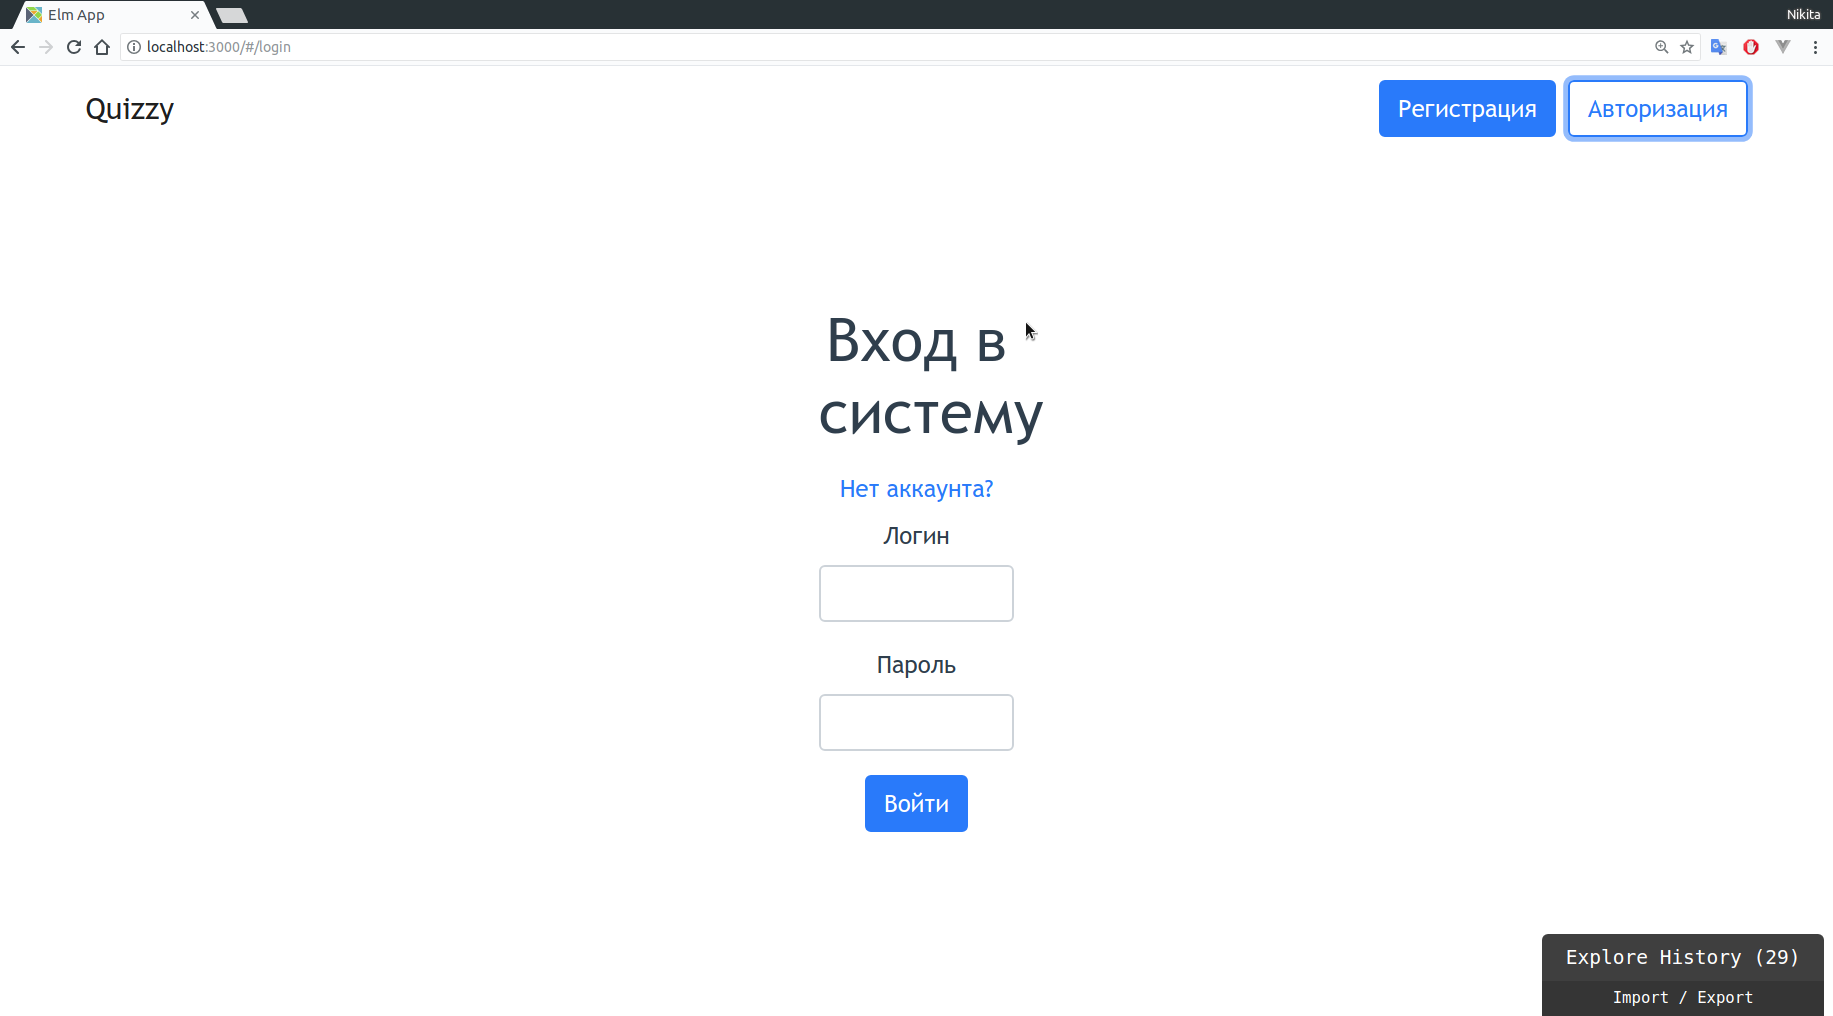
\includegraphics[width=1\textwidth]{img/screens/auth.png}
		\caption{Страница авторизации пользователя}
		\label{scr1}}
\end{figure}
\begin{figure}[ht!]
	\centering{ 
		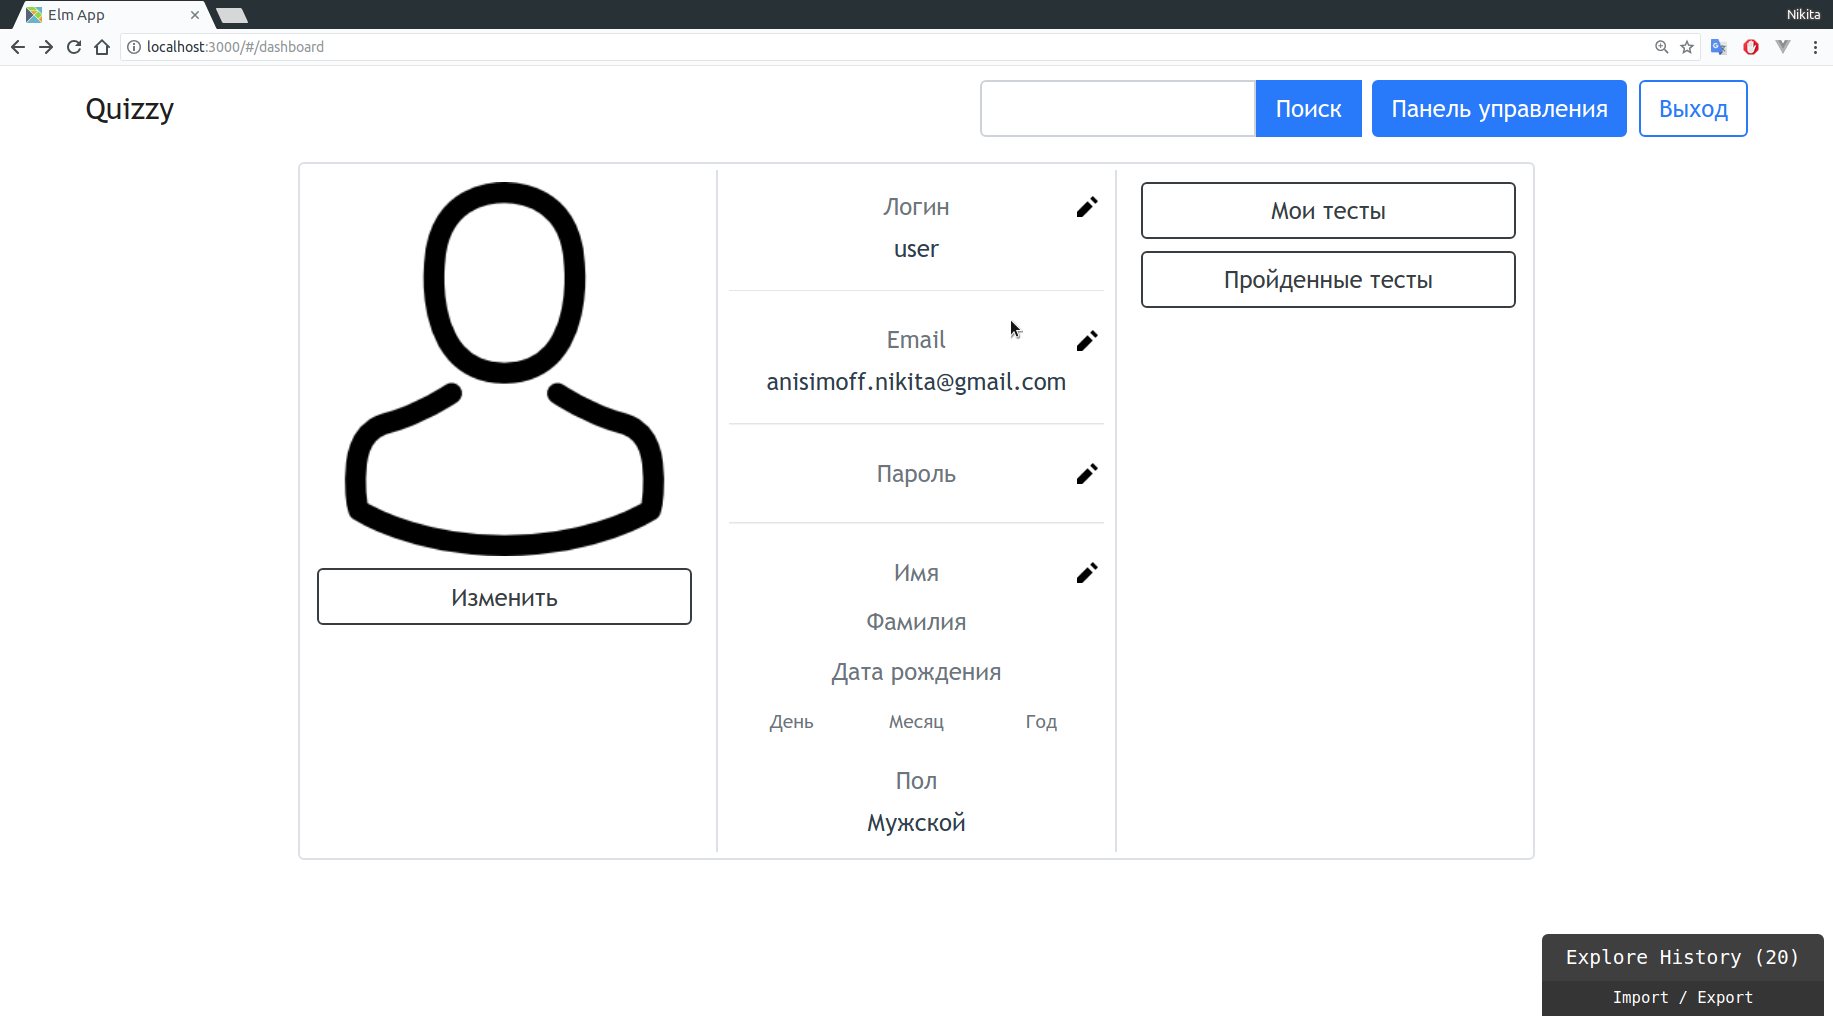
\includegraphics[width=1\textwidth]{img/screens/db.png}
		\caption{Страница пользователя}
		\label{scr2}}
\end{figure}
\begin{figure}[ht!]
	\centering{ 
		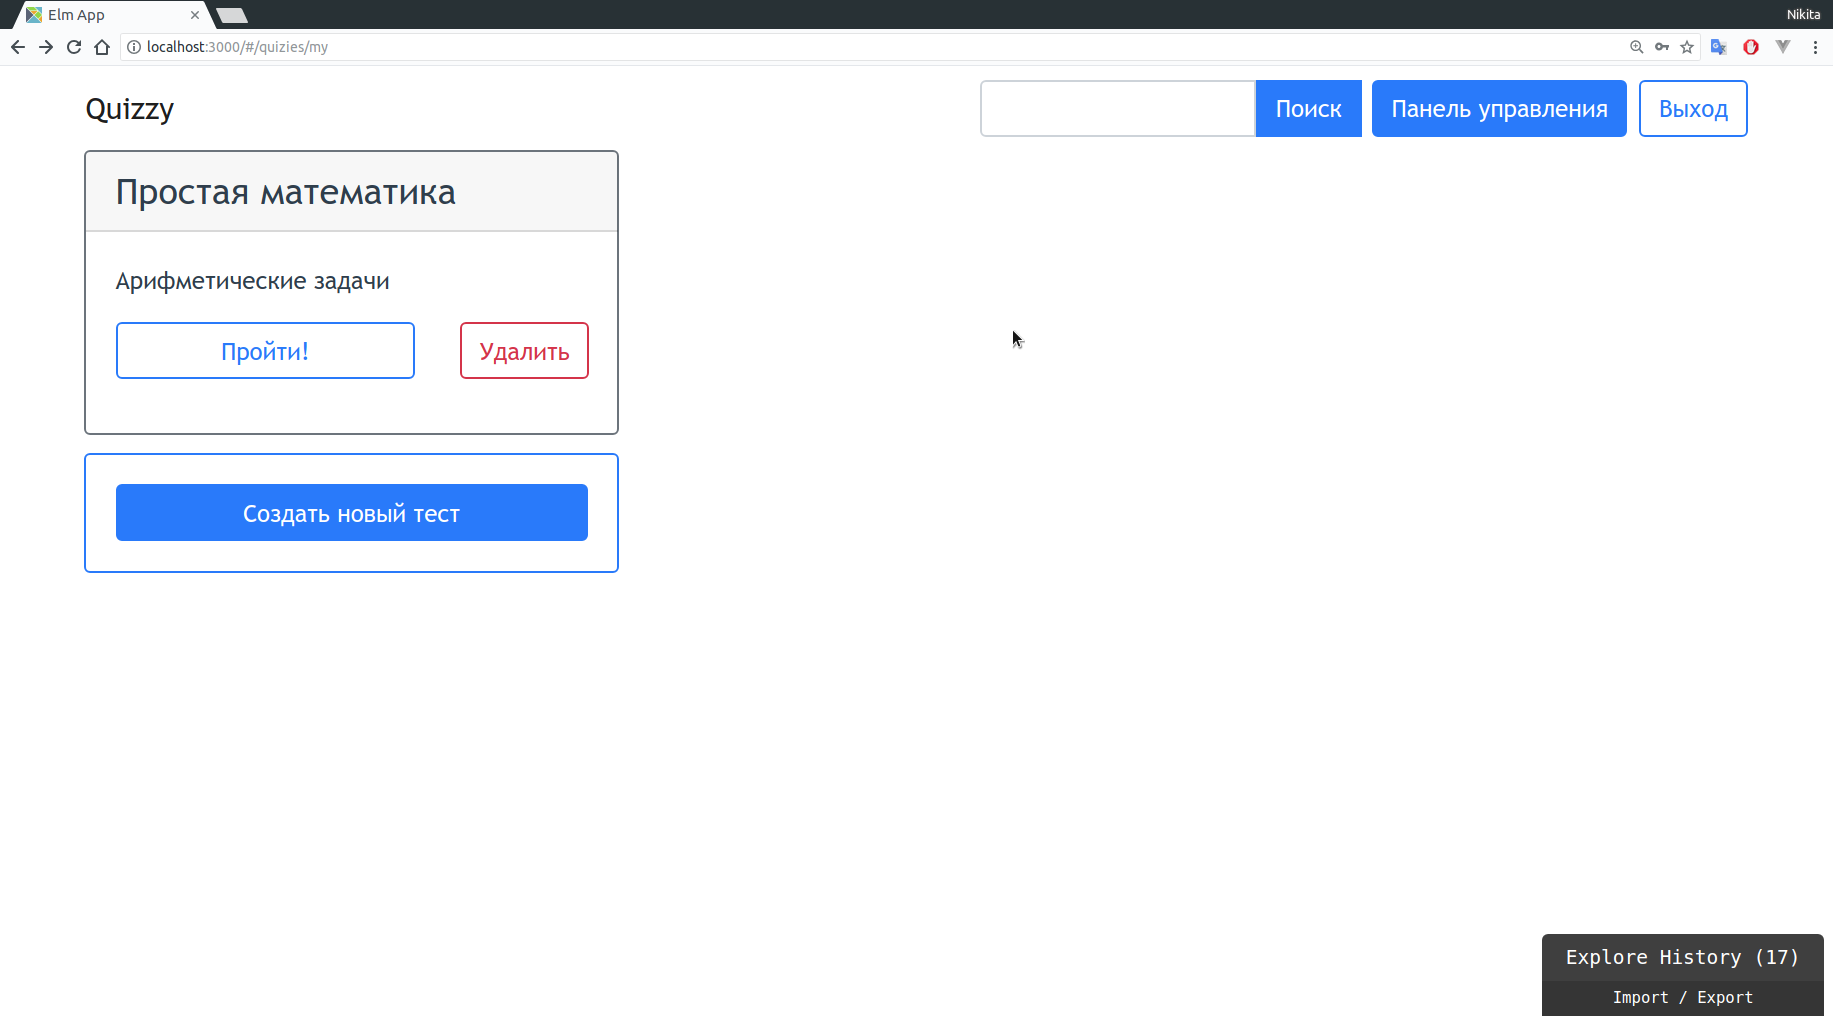
\includegraphics[width=1\textwidth]{img/screens/list.png}
		\caption{Страница управления тестами}
		\label{scr3}}
\end{figure}
\begin{figure}[ht!]
	\centering{ 
		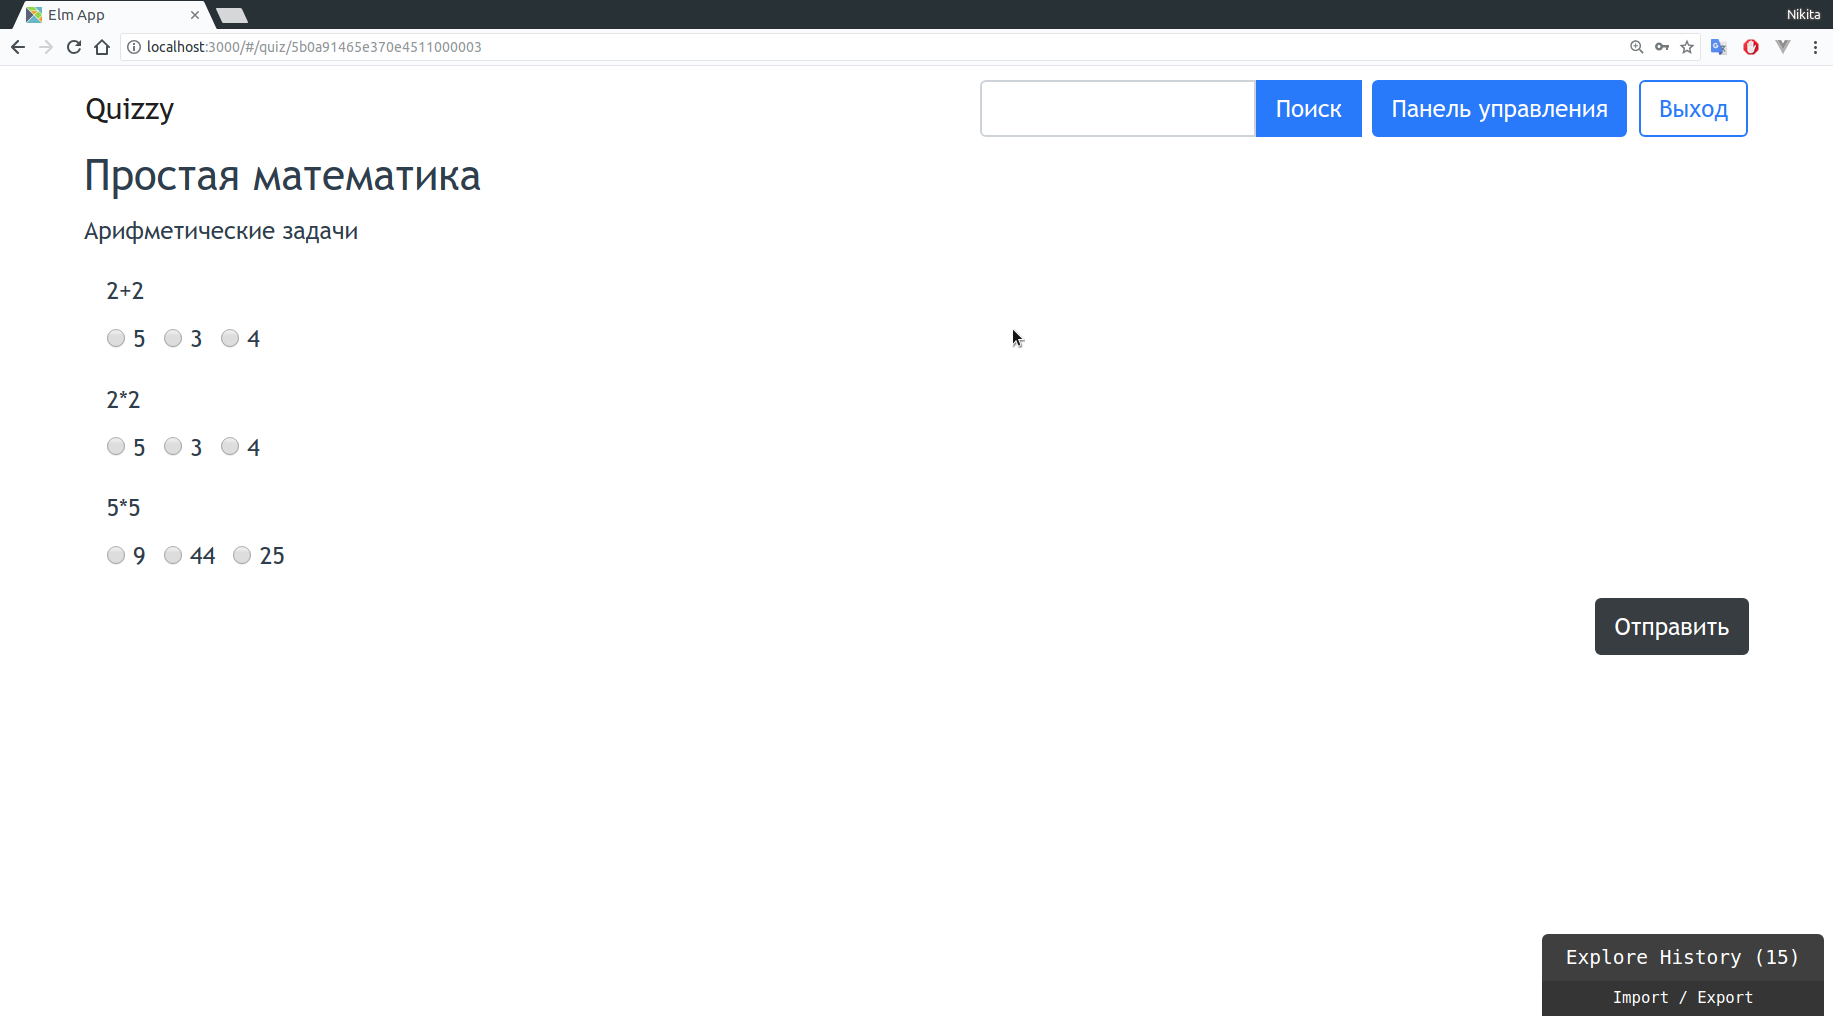
\includegraphics[width=1\textwidth]{img/screens/pass.png}
		\caption{Страница прохождения теста}
		\label{scr4}}
\end{figure}

\clearpage
\section{Выводы}
В качестве документооринтированной базы данных была выбрана MongoDB. Серверная часть написана на языке Haskell, с использованием библиотек Servant и Persistent. Клиент написан на языке Elm. Система разработана и протестирована.